\documentclass[a4paper,12pt]{article}
\usepackage[T2A]{fontenc}
\usepackage[utf8x]{inputenc}
\usepackage[english,russian]{babel}
\usepackage{amssymb,amsfonts,amsmath,mathtext}
\usepackage[unicode]{hyperref}
\usepackage{listings}
\usepackage{graphicx}
\usepackage{float}
\graphicspath{{images/}}
\newcommand{\anonsection}[1]{\section*{#1}\addcontentsline{toc}{section}{#1}}

\begin{document}

% Титульный лист

\begin{titlepage}
\newpage

\begin{center}

\textit{Министерство науки и высшего образования Российской Федерации \\ 
Федеральное государственное бюджетное образовательное \\
учреждение высшего образования \\
«Московский государственный технический университет \\
имени Н.Э. Баумана (национальный исследовательский университет)» \\
(МГТУ им. Н.Э. Баумана) \\}
\hrulefill
\end{center}

\vspace{2em}

\begin{flushleft}
ФАКУЛЬТЕТ <<Информатика и системы управления>> \\
\vspace{0.5em}
КАФЕДРА <<Программное обеспечение ЭВМ и информационные технологии>>
\end{flushleft}


\vspace{8em}

\begin{center}
\LARGE Лабораторная работа №6 \\
\end{center}

\vspace{1.5em}

\begin{center}
\textsc{Муравьиный алгоритм}
\end{center}

\vspace{6em}

\begin{center}
Головнев Н.В.

\vspace{4em}

ИУ7-54Б
\end{center}

\vspace{\fill}

\begin{center}
Москва 2019
\end{center}

\end{titlepage}

\tableofcontents

% Введение

\newpage
\anonsection{ВВЕДЕНИЕ}
Задача коммивояжёра (коммивояжёр — бродячий торговец) заключается в отыскании самого выгодного маршрута, проходящего через указанные города хотя бы по одному разу. В условиях задачи указываются критерий выгодности маршрута (кратчайший, самый дешёвый, совокупный критерий и т. п.) и соответствующие матрицы расстояний, стоимости и т. п. Как правило указывается, что маршрут должен проходить через каждый город только один раз, в таком случае выбор осуществляется среди гамильтоновых циклов. Стандартным методом решения такой задачи является метод полного перебора, однако, он является слишком неэффективным и затратным по времени.\\
Все эффективные (сокращающие полный перебор) методы решения задачи коммивояжёра — методы эвристические. В большинстве эвристических методов находится не самый эффективный маршрут, а приближённое решение. Зачастую востребованы так называемые any-time алгоритмы, то есть постепенно улучшающие некоторое текущее приближенное решение. Одним из таких эвристических алгоритмов является муравьиный алгоритм (оптимизация муравьиной колонией). 

\newpage
\anonsection{ПОСТАНОВКА ЗАДАЧИ}
Цель задачи: Изучить муравьиный алгоритм на материале решения задачи коммивояжера.\\
Задача:\\
\begin{itemize}
\item Описать методы полного перебора и эвристический, основанный на муравьином алгоритме;
\item Реализовать эти методы;
\item Выбрать класс данных, подготовить данные ;
\item Провести параметризацию метода, основанного на муравьином алгоритме;
\item Интерпретировать результаты и сравнить их с результатами метода полного перебора.
\end{itemize}

\newpage
\section{АНАЛИТИЧЕСКАЯ ЧАСТЬ}
\subsection{Описание алгоритма}
Формулировка задачи коммивояжера:\\
Дано $N$ узлов, расположенных на плоскости. Задан входной узел (Вх) и выходной узел (Вых). Необходимо обнаружить кратчайший путь, охватывающий все узлы, начинающийся во входном узле, заканчивающийся в выходном узле и проходящий через каждый узел только 1 раз.\\
\begin{center}
\textbf{Метод полного перебора}
\end{center}
Полный перебор — метод решения задачи путем перебора всех возможных вариантов. Сложность полного перебора зависит от количества всех возможных решений задачи. Если пространство решений очень велико, то полный перебор может не дать результатов в течение нескольких лет или даже столетий.\\

\begin{center}
\textbf{Муравьиный алгоритм}
\end{center}
Муравьиный алгоритм - один из эффективных полиномиальных алгоритмов (эвристический) для нахождения приближённых решений задачи коммивояжёра, а также решения аналогичных задач поиска маршрутов на графах. Суть подхода заключается в анализе и использовании модели поведения муравьёв, ищущих пути от колонии к источнику питания.\\
Пусть города заданы матрицей кратчайших расстояний.\\
У муравья присутствуют 3 чувства:
\begin{enumerate}
\item Зрение (определяет длину ребра)
\item Обоняние (чует феромон)
\item Память (запоминает пройденный маршрут)
\end{enumerate}
Пусть феромон на ребре $D_{ij}$ в момент времени $t = \tau_{ij}$. На старте инициализируется матрица $\tau$ константами.\\
Находясь в городе $i$ муравей $k$  принимает решение о выборе случайного города $j$ по следующему правилу\cite{Shtobva}\\
\begin{equation}\label{equations:equation1}
P_{k,ij} = \left\{
\begin{array}{ll}
\frac{\tau_{ij}(t)^\alpha * (\eta_{ij})^\beta}{\sum_{q \in C}(\tau_{iq}(t)^\alpha * (\eta_{iq})^\beta)} & j \in C \\
0 & j \in C \\
\end{array}
\right.
\end{equation}
Здесь:\\
$P_{k,ij}$ - вероятность того, что муравей $k$ будет двигаться из города $i$ в город $j$,\\
$C$ - множество городов, которые муравей ещё не посещал,\\
$\tau_{ij}$ - кол-во феромонов на ребре $ij$,\\
$\alpha$ - параметр, контролирующий влияние $\tau_{ij}$,\\
$\eta_{ij}$ - привлекательность ребра ($\eta_{ij} = \frac{1}{D_{ij}}$),\\
$\beta$ - параметр, контролирующий влияние $\eta_{ij}$.\\
Обновление феромонов:\\
\begin{equation}\label{equations:equation2}
\tau_{ij} = (1 - \rho)\tau_{ij} + \Delta\tau_{ij}
\end{equation}
Где:\\
$\tau_{ij}$ - воличество феромона на ребре $ij$,\\
$\rho$ - скорость испарения феромона,\\
$\Delta\tau_{ij}$ - количество отложенного муравьем феромона, обычно определяется как:\\
\begin{equation}\label{equations:equation3}
\Delta\tau_{ij}^k = \left\{
\begin{array}{ll}
\frac{Q}{L_k} & \text{if ant } k \text{ travels on edge } ij\\
0 & otherwise 
\end{array}
\right.
\end{equation}
$L_k$ - стоимость пути, пройденного $k$-м муравьем, $Q$ - параметр, имеющий значение порядка длины оптимального пути.\\
Псевдокод решения задачи коммивояжёра при помощи муравьиного алгоритма\cite{Shtobva}:\\
1. Ввод матрицы расстояний $D$\\
2. Инициализация параметров алгоритма – $Q$,$\beta$,$\alpha$\\
3. Инициализация рёбер – присвоение видимости $\eta_ij$ и начальной концентрации феромона \\
4. Размещение муравьёв в случайно выбранные города без совпадений \\
5. Выбор начального кратчайшего маршрута\\
6. Цикл по времени жизни колонии $t \leftarrow 1$ to $t_{max}$ \\
7.  Цикл по всем муравьям $k \leftarrow 1$ to $m$\\
8.  Построить маршрут $T_k(t)$ по правилу \eqref{equations:equation1} и рассчитать длину $L_k(t)$\\
9.  конец цикла по муравьям \\
10.  Проверка всех на лучшее решение по сравнению с $L^*$\\
11.  Вслучае если решение $L_k(t)$ лучше, обновить $L^*$ и $T^*$\\
12.  Цикл по всем рёбрам графа \\
13.  Обновить следы феромона на ребре по правилам \eqref{equations:equation2} и \eqref{equations:equation3}\\ 
14.  конец цикла по рёбрам\\
15. конец цикла по времени\\
16. Вывести кратчайший маршрут $T^*$  и его длину $L^*$

\newpage
\subsection{Вывод}
В данном разделе были описаны принципы работы алгоритмов, решающие задачу коммивояжера - муравьиный алгоритм и алгоритм, использующий полный перебор. На основе этих принципов теперь можно написать приложение, реализующее поиск оптимального расстояния для обхода всех городов.

% Конструкторская часть

\newpage
\section{КОНСТРУКТОРСКАЯ ЧАСТЬ}

\subsection{Разработка алгоритма}
На вход у муравьиного алгоритма передаются в качестве параметров:
\begin{enumerate}
\item Матрица расстояний, матрица феромонов и матрица со значениями обратных расстояний;
\item Количество узлов;
\item Количество муравьев;
\item Муравьи (специальная структура, в которую записывается текущее расстояние и путь);
\item Ссылка на результат (переменная результата имеет такую же стуруктуру, что и муравьи);
\item Параметры муравьиного алгоритма.
\end{enumerate}
Возвращаемое значение: код ошибки (0 в случае успеха, иначе отрицательное значение). \\
Побочные эффекты:
Изменяется содержимое результата (сохраняется путь в переменную результата).

На вход у алгоритма, использующего метод полного перебора, в качестве параметров передаются:
\begin{enumerate}
\item Матрица расстояний;
\item Количество узлов;
\item Ссылка на результат;
\end{enumerate}
Возвращаемое значение: код ошибки (0Гр в случае успеха, иначе отрицательное значение). \\
Побочные эффекты:
Изменяется содержимое результата (сохраняется путь в переменную результата).

\newpage
\subsection{Вывод}
На основе аналитических данных были разработаны требования к разрабатываемому алгоритму.

\newpage
\section{ТЕХНОЛОГИЧЕСКАЯ ЧАСТЬ}
\subsection{Требования к программному обеспечению}
Программа должна работать на операционной системе Arch Linux. Пользователь должен иметь возможность взаимодействовать с программой, используя консоль или терминал. На вход программе пользователь подает:
\begin{itemize}
\item Имя файла с описанием матрицы расстояний;
\item Параметры муравьиного алгоритма (коэффициенты, время жизни и тд...);
\end{itemize}
На выходе программа должна печатать значения найденных кратчайших путей (результат решения задачи коммивояжёра) и длины этих путей.\\
Программа должна проверять вводимые данные на корректность, в случае некорректности, выслать предупреждение.
Матрица в файле описывается так:
\begin{itemize}
\item на первой строке записывается размер матрицы (длина стороны квадратной матрицы);
\item на остальных строках записываются значения матрицы.
\end{itemize}
Матрица расстояний должна описывать полносвязный неориентированный граф.

\newpage
\subsection{Средства реализации}
Для реализации данных алгоритмов был выбран язык программирования С, компилятор gcc и некоторые функции из библиотеки glibc (memcpy, malloc и тд...). \\
Основные особенности Си:
\begin{itemize}
\item простая языковая база, из которой в стандартную библиотеку вынесены многие существенные возможности, вроде математических функций или функций работы с файлами;
\item ориентация на процедурное программирование;
\item система типов, предохраняющая от бессмысленных операций;
\item использование препроцессора для абстрагирования однотипных операций;
\item доступ к памяти через использование указателей;
\item небольшое число ключевых слов;
\item передача параметров в функцию по значению, а не по ссылке (передача по ссылке эмулируется с помощью указателей);
\item наличие указателей на функции и статических переменных;
\item области видимости имён;
\item структуры и объединения — определяемые пользователем собирательные типы данных, которыми можно манипулировать как одним целым.
\end{itemize}

\newpage
\subsection{Листинг кода}
Ниже приведены реализации алгоритмов на С.\\
\lstdefinestyle{customc}{
  belowcaptionskip=1\baselineskip,
  breaklines=true,
  frame=L,
  xleftmargin=\parindent,
  language=C,
  showstringspaces=false,
  basicstyle=\footnotesize\ttfamily
}

\lstinputlisting[captionpos=b, caption=\label{listings:listing1}Реализация муравьиного алгоритма, style=customc]{listing1.c}
\newpage
\lstinputlisting[captionpos=b, caption=\label{listings:listing2}Реализация алгоритма полного перебора, style=customc]{listing2.c}

\newpage
\subsection{Вывод}
Используя язык программирования C, в ходе практической работы была спроектирована и написана реализация муравьиного алгоритма (ACO).

\newpage
\section{ЭКСПЕРИМЕНТАЛЬНАЯ ЧАСТЬ}
\subsection{Характеристики аппаратного и программного обеспечения}
% Часть которую никогда нельзя менять
Тестирование приложения проводилось на машине со следующими характеристиками:\\
\begin{itemize}
\item Процессор Intel® Core™ i7-7700HQ;
\item Оперативная память 16 ГБ;
\item Операционная система - Arch Linux с рабочим окружением Cinnamon.
\end{itemize}

\newpage
\subsection{Примеры работы}
На рис. \ref{images:example}, предсавленном ниже, демонстрируется работа приложения. Запуск приложения осуществляется из эмулятора терминала в Arch Linux.
\begin{figure}[h]
\center{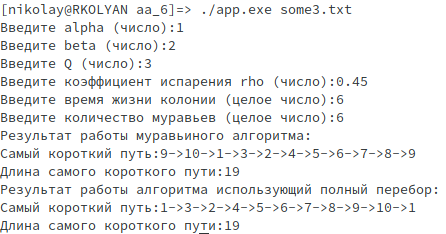
\includegraphics[scale=0.75]{example1.png}}
\caption{Пример работы приложения}
\label{images:example1}
\end{figure}
\begin{figure}[h]
\center{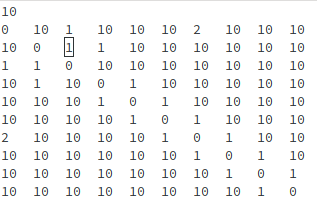
\includegraphics[scale=0.9]{example2.png}}
\caption{Содержимое файла some3.txt}
\label{images:example2}
\end{figure}

\newpage
\subsection{Оценка времени выполнения}
На рис. \ref{graphics:graphic1} представлен график зависимости количества всех перебираемых комбинаций, использующиеся алгоритмами для высчитывания минимального пути.
\begin{figure}[h]
\center{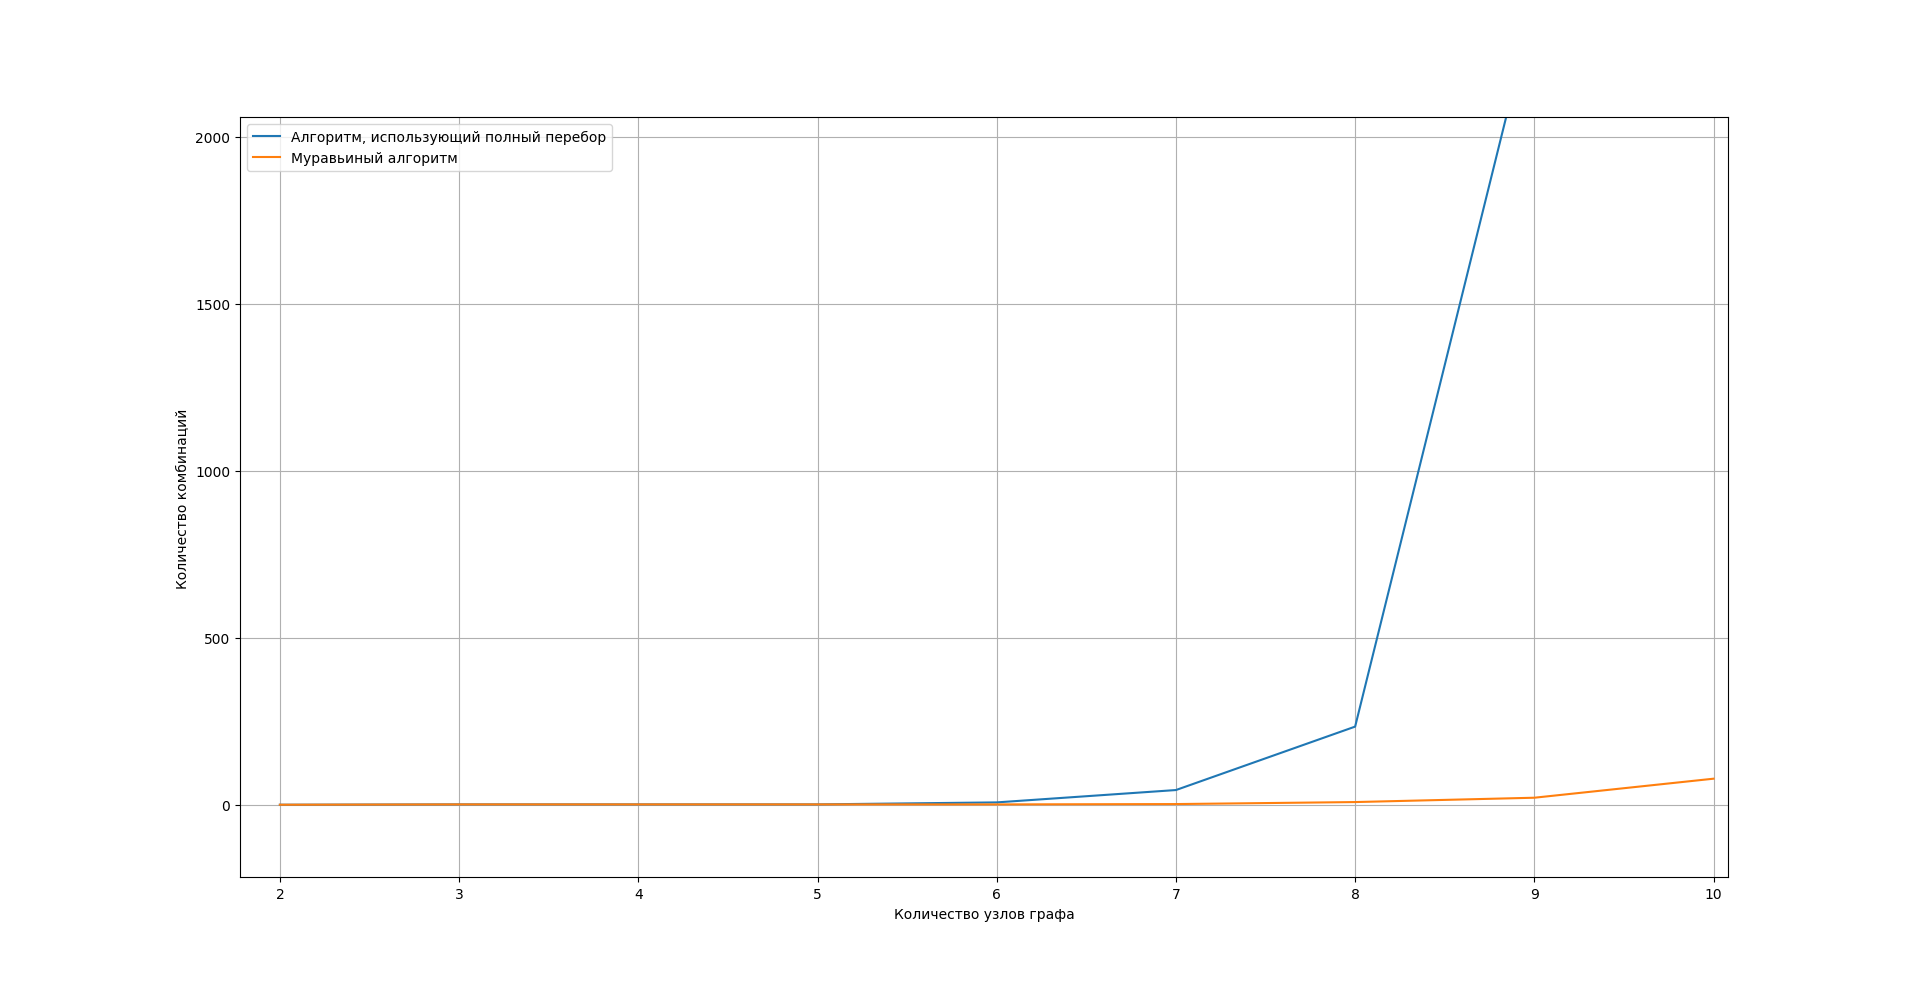
\includegraphics[scale=0.3]{graphics.png}}
\caption{График}
\label{graphics:graphic1}
\end{figure}

\newpage
\subsection{Вывод}
Исходя из данных, полученных в результате эксперимента, можно сделать вывод, что муравьиный алгоритм значительно выигрывает у алгоритма, использующий метод полного перебора. При большом количестве узлов графа (как показано на графиках), алгоритм полного перебора \textbf{значительно} неэффективен.

\newpage
\anonsection{ЗАКЛЮЧЕНИЕ}
Данные алгоритмы могут быть использованы не только как алгоритмы решения задачи коммивояжёра, но и как алгоритмы нахождения кратчайшего расстояния между двумя вершинами графа. Например, искать текущий минимальный маршрут между двумя городами имея определенную сеть дорог.
Муравьиный алгоритм (вернее, его модификации) на сегодняшний день признан одним из самых эффективных алгоритмов, решающих различные транспортные проблемы (пробки в городах, отсутствие прямого пути между пунктами назаначения и тд...).

\newpage
\anonsection{СПИСОК ИСТОЧНИКОВ}
\begingroup
\renewcommand{\section}[2]{}
\begin{thebibliography}{2}
\bibitem{Shtobva} Штовба С. Д. Муравьиные алгоритмы, Exponenta Pro. Математика в приложениях. 2004. № 4
\bibitem{Habr} Хабр, муравьиные алгоритмы - \url{https://habr.com/ru/post/105302/}
\end{thebibliography}
\endgroup

\end{document}
